\documentclass[12pt]{memoir}

\def\nsemestre {I}
\def\nterm {Spring}
\def\nyear {2023}
\def\nprofesor {Jeff Achter}
\def\nsigla {MATH519}
\def\nsiglahead {Complex Analysis}
\def\nlang {ENG}
\input{../../headerVarillyDiff}

\begin{document}
%\clearpage
\maketitle
%\thispagestyle{empty}
{\small
\setlength{\parindent}{0em}
\setlength{\parskip}{1em}

This course is an introduction to analytic functions of a single complex variable.  The subject is beautiful.-- it turns out that a function with a complex derivative is highly structured -- and enjoys a give and take with many other areas of mathematics.

\subsubsection*{Requirements}
Knowledge of convergence of sequences, series: limits, continuity, differentiation, integration of one-variable functions is required.
}
\newpage
\tableofcontents
%\begin{multicols}{2}
\chapter{First Midterm}

\section{Interim| HW1}

\begin{Ej}[1.1 Stein \& Shakarchi]
Describe geometrically the sets of points $z$ in the complex plane defined by the following relations:
\begin{enumerate}
    \itemsep=-0.4em
    \item $|z-z_1|=|z-z_2|$ where $z_1,z_2\in\bC$.
    \item $1/z=\ov z$.
    \item $\Re(z)=3$
    \item $\Re(z)>c$, (resp.,$\geq c$) where $c\in\bR$.
    \item $\Re(az+b)>0$ where $a,b\in\bC$.
    \item $|z|=\Re(z)+1$.
    \item $\Im(z)=c$ with $c\in\bR$.
\end{enumerate}
\end{Ej}

\begin{ptcbr}
    \begin{enumerate}[i)]
        \itemsep=-0.4em
        \item The first set is the set of points at the same distance from $z_1$ and $z_2$. If we consider the line segment $z_1z_2$, then the set in question is the bisector of that line segment.
        \item Note that
        $$1/z=\ov z\iff 1=\ov zz\iff 1=|z|^2\iff 1=|z|,$$
        thus the set is the unit circle.
        \item The set is a perpendicular line to the real axis at $z=3$.
        \item This infinite set is an infinite half plane to the right (but not including) of the line $z=c$. In the other case, we do include the line in question.
        \item Let us rephrase this inequality in terms of real numbers. Call $a=a_1+ia_2$, $b=b_1+ib_2$ and $z=x+iy$. Then 
        $$\Re(az+b)=\Re[a_1 x - a_2 y + b_1 + i (a_2 x +  a_1 y +  b_2)],$$
        thus our desired inequality is true whenever $a_1 x - a_2 y + b_1>0$. Solving for $y$ we get $y>(a_1x+b_1)/a_2$, which is the half plane located above the line $y=(a_1x+b_1)/a_2$.
        \item The equation in question is equivalent to 
        $$\Re(z)^2+\Im(z)^2=(\Re(z)+1)^2.$$
        To ease the notation, assume $z=x+iy$. Then the equation reads 
        $$x^2+y^2=x^2+2x+1\iff y^2=2x+1\iff x=(y^2-1)/2.$$
        It holds the the parabola in question contains the points which satisfy the equation.
        \item This set is a line parallel to the real axis at $z=c$
    \end{enumerate}
\end{ptcbr}

\begin{Ej}
    Do the following:
    \begin{enumerate}[i)]
        \itemsep=-0.4em
        \item Show that the complex conjugation map $\kp:\bC\to\bC,\ z\mapsto\ov z$ is an involution, i.e., a ring homomorphism such that $\kp\circ\kp=\id$.
        \item Suppose $a\in\bR,\ z\in\bC$. Show that 
        $$\Re(az)=a\Re(z),\word{and}\Im(az)=a\Im(z).$$
    \end{enumerate}
\end{Ej}

\begin{ptcbr}
    Let us take $z=x+iy$ with $x,y\in\bR$.
    \begin{enumerate}[i)]
        \itemsep=-0.4em
        \item We have $\ov z=x+i(-y)=x-iy$. Once more we get $\ov{\ov z}=x-i(-y)=x+iy=z$. Thus $\ov{\ov z}=z$ for any $z\in\bC$. In conclusion $\ov{\ov \.}=\id$.
        \item It holds that 
        \begin{align*}
            &\Re(az)=\Re(ax+aiy)=ax=a\Re(z),\\
            &\Im(az)=\Im(ax+aiy)=ay=a\Im(z).
        \end{align*}
    \end{enumerate}
\end{ptcbr}

\begin{Ej}
    Do the following:
    \begin{enumerate}[i)]
        \itemsep=-0.4em
        \item Prove that $|z+w|^2=|z|^2+|w|^2+2\Re(z\ov w)$.
        \item Use this to prove the parallelogram rule: $|z+w|^2+|z-w|^2=2(|z|^2+|w|^2)$.
    \end{enumerate}
\end{Ej}

\begin{ptcbr}
    \begin{enumerate}[i)]
        \itemsep=-0.4em
        \item Note that 
        $$|z+w|^2=(z+w)\ov{(z+w)}=(z+w)(\ov z+\ov w)=z\ov{z}+w\ov{z}+z\ov{w}+w\ov w.$$
        The number $w\ov z$ is the conjugate of $z\ov w$, and summing a number and its conjugate returns twice its real part. Thus we get the desired identity. 
        \item As the past identity holds for all complex numbers, it holds when $w=-w$. This means that 
        $|z-w|^2=|z|^2+|-w|^2+2\Re(z(\ov{-w}))=|z|^2+|w|^2-2\Re(z\ov w)$
        and summing this together with the first identity gives us the parallelogram law.
    \end{enumerate}
\end{ptcbr}

\begin{Ej}[1.5 Stein \& Shakarchi]
    A set $\Om$ is said to be pathwise connected if any two points in $\Om$ can be joined by a (piecewise-smooth) curve entirely contained in $\Om$. The purpose of this exercise is to prove that an open set $\Om$ is pathwise connected if and only if $\Om$ is connected.
    \begin{enumerate}[i)]
        \itemsep=-0.4em
        \item Suppose first that $\Om$ is open and pathwise connected, and that it can be written as $\Om$ = $\Om_1\cup\Om_2$ where $\Om_1$ and $\Om_2$ are disjoint non-empty open sets. Choose two points $w_1\in\Om_1$ and $w_2\in\Om_2$ and let $\ga$ denote a curve in $\Om$ joining $w_1$ to $w_2$. Consider a parametrization $z:\bonj{0,1}\to\Om$ of this curve with $z(0) = w_1$ and $z(1) = w_2$, and let
        $$t_\ast = \sup_{0\leq t\leq 1}\set{t\:\forall s [(0\leq s<t)\To (z(s)\in\Om_1)]}.$$
        Arrive at a contradiction by considering the point $z(t_\ast)$.
        \item Conversely, suppose that $\Om$ is open and connected. Fix a point $w\in\Om$ and let $\Om_1\subseteq\Om$ denote the set of all points that can be joined to $w$ by a curve contained in $\Om$. Also, let $\Om_2\subseteq\Om$ denote the set of all points that cannot be joined to $w$ by a curve in $\Om$. Prove that both $\Om_1$ and $\Om_2$ are open, disjoint and their union is $\Om$. Finally, since $\Om_1$ is non-empty (why?) conclude that $\Om$ = $\Om$1 as desired.
    \end{enumerate}
    \end{Ej}

\begin{ptcbr}
    \begin{enumerate}[i)]
        \itemsep=-0.4em
        \item 
        \iffalse
        Recall first, that by definition of supremum we have that if $S$ is our set, then 
        $$\exists s\in S(s>t_\ast-\eps)$$
        for $\eps>0$. Following the idea, we consider the point $z(t_\ast)$. We have two options to place $z(t_\ast)$, either in $\Om_1$ or $\Om_2$.\par 
        Let's start by definition of supremum \red{FINISH}
        Let us proceed as mentioned by assuming $\Om$ is disconnected.
        For the point $z(t_\ast)$ we have two options, either it's in $\Om_1$ or $\Om_2$.\par 
        If it ocurred that $z(t_\ast)\in\Om_1$ then, as $\Om_1$ is open, there exists $r>0$ such that $B(z(t_\ast),r)\subseteq \Om_1$. 
        \fi 
        We will proceed using a topological argument instead of a metric one. As the function $\ga$ is continuous, it pulls back $\Om_1$ and $\Om_2$ into $[0,1]$ as open sets. However, as the sets are disjoint, their inverse images are disjoint as well. In other words, we have found two open disjoint sets which separate $[0,1]$: 
        $$[0,1]=\ga^{-1}[\Om_1]\cupdot\ga^{-1}[\Om_2].$$
        But this is impossible because $[0,1]$ is a connected set. Thus, our assumption that $\Om$ was disconnected must be false. We conclude that path-connectedness implies connectedness.
        \item Take $\Om_1,\Om_2$ as in the statement. Then $\Om_1$ is non-empty as $w\in\Om_1$ because it's connected to itself through a trivial path. Suppose now that $z\in\Om_1$ and that $d(z,\del\Om_1)>r>0$. Take $x\in B(z,r)$, then there exists a line-segment between $z$ and $x$ and there's a smooth curve which connects $z\in\Om_1$ with $w$. Thus the piecewise-continuous path from $x$ to $z$ and from $z$ to $w$ is a path which connects $x$ and $w$. As $x$ is arbitrary, it follows that $B(z,r)\subseteq \Om_1$, and thus $\Om_1$ is open.\par 
        Formally, if $\ga:[0,1]\to\Om_1$ is the map which parametrizes the curve between $z$ and $w$ and $r:[0,1]\to B(z,r)$ is the map $t\mapsto tz+(1-t)x$, then the curve from $x$ to $w$ is parametrized by the function 
        $$f=\begin{cases}
            2tz+(1-2t)x,\ t\in[0,1/2],\\
            \ga(2t-1),\ t\in[1/2,1].
        \end{cases}$$
        On the other hand take a point $z\in\Om_2$ and let $d(z,\del\Om_2)>r>0$. Consider a point $x\in B(z,r)$ and assume by way of contradiction that such $x$ can be connected to $w$ by a curve which can be parametrized by a smooth function $\ga$. As the ball is convex, we can connect $z$ to $x$ and then to $w$ creating a path between $z$ and $w$. This is impossible as $z$ cannot be connected to $w$ by a path, thus our assumption must be false. It holds that $x$ cannot be connected to $w$ by a path and thus $x\in\Om_2$. Therefore $\Om_2$ is also open. We conclude that $\Om=\Om_1\cup\Om_2$ is a union of two disjoint open sets, and since $\Om$ is connected, it must hold that $\Om_2$ is empty. We conclude that $\Om$ is path-connected. 
    \end{enumerate}
\end{ptcbr}

\begin{Ej}[1.7 Stein \& Shakarchi]
    The family of mappings introduced here plays an important role in complex analysis. These mappings, sometimes called \textbf{Blaschke factors}, will reappear in various applications in later chapters.
    \begin{enumerate}[i)]
        \itemsep=-0.4em
        \item Let $z,w\in\bC$ such that $\ov{z}w\neq 1$. Prove that 
        $$\left|\frac{w-z}{1-\ov w z}\right|<1$$
        if $|z|<1$ and $|w|<1$, and also that 
        $$\left|\frac{w-z}{1-\ov w z}\right|=1$$
        if $|z|=1$ or $|w|=1$. \hint{Why can one assume that $z$ is real? I then suffices to prove that $(r-w)(r-\ov w)\leq (1-rw)(1-r\ov w)$ with equality for appropriate $r$ and $|w|$.}\aside{Here is an alternate approach, which you may use if you like. Fix $w\in\bC$ with $w<1$, and consider the function $z\mapsto \frac{w-z}{1-\ov w z}$. What is $\ov{f(z)}$? By computing $f(z)\ov{f(z)}$, show that $|z|=1$ implies $|f(z)|=1$. Find a point $z$ with $|z|<1$ such that $|f(z)|<1$. Since $f$ is continuous, this shows that $f$ takes the unit disc to itself. (Why?)}
        \item Prove that for a fixed $w\in\bD$, the mapping $F\:z\mapsto\frac{w-z}{1-\ov w z}$ satisfies the following:
        \begin{enumerate}[a)]
            \itemsep=-0.4em
            \item $F$ maps the unit disc to itself (that is, $F:\bD\to\bD$), and is holomorphic.
            \item $F$ interchanges $0$ and $w$. 
            \item $|F(z)|=1$ if $|z|=1$.
            \item $F$ is bijective. \hint{Calculate $F\circ F$.}
        \end{enumerate}
    \end{enumerate}
    \end{Ej}

    \begin{ptcbr}
        \begin{enumerate}[i)]
            \itemsep=-0.4em
            \item The inequality in question is equivalent to 
            $$0\leq|w-z|<|1-\ov wz|.$$
            Since the quantities are positive, we can square them and preserve the order. It holds that 
            $$0\leq|w-z|^2<|1-\ov wz|^2\iff 0\leq (w-z)\ov{(w-z)}<(1-\ov wz)\ov{(1-\ov wz)},$$
            Simplifying this expression we get 
            \begin{align*}
                &(w-z)(\ov w-\ov z)<(1-\ov wz)(1-w\ov z)\\
                \iff&w\ov w-w\ov z -z\ov w+z\ov z<1-w\ov z-\ov wz+\ov wzw\ov z\\
                \iff&|w|^2+|z|^2<1+|w|^2|z|^2\\
                \iff&0<(1-|w|^2)(1-|z|^2).
            \end{align*}
            The inequality is true whenever both moduli are less than one, and whenever either is one equality is achieved.
            \item Now we suppose $w\in\bD$ which means that $|w|<1$. Taking $z\in\bD$ and applying $F$ gives us the quantity $\frac{w-z}{1-\ov w z}$ which by the previous argument, has modulus less than $1$ whenever $w,z$ do.\par 
            The function $F$ is holomorphic because it is a quotient of holomorphic functions. The denominator is never zero inside the domain because that would mean that $1=\ov w z$. And taking moduli in both sides of the equation gives us 
            $$1=|1|=|w||z|<1$$
            which is impossible.\par 
            Now $F(0)=\frac{w-0}{1-0}=w$ and $F(w)=\frac{w-w}{1-|w|^2}=0$. The denominator in the last expression is never zero because $|w|<1$.\par 
            By the second part of the previous argument it holds that $|z|=1$ immediately gives us $|F(z)|=1$. And finally we will see that $F$ is an involution:
            $$F(F(z))=F\left(\frac{w-z}{1-\ov w z}\right)=\frac{w-\left(\frac{w-z}{1-\ov w z}\right)}{1-\ov w\left(\frac{w-z}{1-\ov w z}\right)}.$$ 
            Homogenizing and clearing denominators we get 
            $$\frac{w(1-\ov wz)-w+z}{1-\ov w z-\ov w(w-z)}=\frac{-w\ov wz+z}{1-\ov ww}=\frac{(-w\ov w+1)z}{1-\ov ww}=z.$$
            This means that $F$ is it's own inverse and therefore, $F$ is bijective. 
        \end{enumerate}
    \end{ptcbr}
\section{Day 1| 20230120}

\subsection{The Complex Numbers}

To construct the complex numbers we take the real numbers, adjoin a variable and mod out by $\genr{x^2+1}$. We can also define $\bC$ as $\set{a+bi:\ a,b\in\bR}$ with the property $i^2=-1$. This means that we can multiply complex numbers in the following way:
$$(a+bi)(c+di)=ac+(bc+ad)i+bdi^2=(ac-bd)+(ad+bc)i.$$
Also as $x^2+1$ is irreducible in $\bR[x]$, $\bC$ is a finite field extension of $\bR$ of degree 2. As a 2-dimensional vector space $\set{1,i}$ is a basis for $\bC$.\par 
The map $a+bi\mapsto\twobyone{a}{b}$ is not a ring homomorphism, it's a bijection with a bit of structure. The map $z\mapsto \al z$, when $\al=a+bi$, is a linear map with the following action over the basis 
\begin{align*}
    &\al\. 1=\al\To[\al]\twobyone{1}{0}=\twobyone{a}{b}\\
    &\al\. i=-b+ai\To[\al]\twobyone{0}{1}=\twobyone{-b}{a}
\end{align*}
which means that $[\al]=\twobytwo{a}{-b}{b}{a}$. The converse, if we have a $\bR$-linear transformation, then it's $\bC$-linear if and only if it looks like $\twobytwo{a}{-b}{b}{a}$.

\begin{Def}
The \term{complex conjugation} map is $a+bi\mapsto a-bi$, or $z\mapsto\ov z$.
\end{Def}

This map is $\bR$-linear but not $\bC$-linear. 

\begin{Ex}
For $\al=a+bi$, we have 
$$\ov{2\al}=\ov{2(a+bi)}=\ov{2a+2bi}=2a-2bi=2\ov{al}.$$
Whereas if instead 
$$\ov{i\al}=\ov{ai-b}=-b-ai\neq i\ov{\al}=b+ai.$$
\end{Ex}

As a $\bR$-linear map, we can identify with the matrix $\twobytwo{1}{0}{0}{-1}$. By looking at the shape of this matrix we can see that it is not $\bC$-linear.

\begin{Lem}
The map $z\mapsto\ov z$ is a ring homomorphism
\end{Lem}

\begin{ptcbp}
$\ov{z+w}=\ov z+\ov w$ and $\ov{zw}=\ov z\ov w$.
\end{ptcbp}

With the complex conjugation we can pick out the real and imaginary parts of $\al=a+bi$. 
$$\al+\ov\al=2\Re(\al),\quad \al-\ov\al=2i\Im(\al)$$
\subsubsection{A Notion of Size}
Can't do geometry without one. Notice that for $z=a+bi$
$$z\ov z=a^2+b^2>0.$$
From a complex number we have extracted a positive quantity.

\begin{Def}
    The \term{complex modulus} of $z$ is $|z|=\sqrt{z\ov z}$.
\end{Def}

The fact that every number has $n$ roots is very important in complex analysis.\par 
As a vector in the plane, the norm of $z$ is $|z|$
\begin{center}
    INC FIG
\end{center}
This means that $a+bi\mapsto\twobyone{a}{b}$ is an isometry. In this sense the distance between two complex numbers is $d(z,w)=|z-w|$.

\subsubsection{Polar Coordinates (\emph{ad hoc})}

For $\te\in\bR$, define 
$$\exp(i\te)=e^{i\te}=\cos(\te)+i\sin(\te)\To |\exp(i\te)|=\sqrt{\cos^2(\te)+\sin^2(\te)}=1.$$
Every point in the unit circle is of the form $e^{i\te}$ and vice-versa.
\begin{center}
    INC FIG
\end{center}
For non-zero complex numbers, $z=|z|e^{i\te}$ for some $\te$.

\begin{Def}
    For a complex number $z=re^{i\te}$, an \term{argument} of $z$ is $\te$. 
\end{Def}
To have a well defined function, we mod out by multiples of $2\pi$: $$\arg:\bC\less\set{0}\to\quot{\bR}{2\pi\bZ},$$
and we obtain a group isomorphism. In general, ``lengths multiply, angles add.''\par 
For inverses if $z=re^{i\te}$, then $\frac{1}{z}=\frac1re^{-i\te}$.

\begin{Def}
    The \term{upper-half plane} is $\bH=\set{\Im(z)>0}$.
\end{Def}

\begin{Lem}
    If $H$ is a half plane $\Im(z-\bt/\ga)>0$
\end{Lem}

\section{Day 2| 20230123}

Recall the complex conjugation map and the modulus of a complex number. This gives us an isometry between $\bR^2$ and $\bC$. Let us prove the lemma from last time. 

\begin{Lem}
    If $H\subseteq\bC$ is a half plane, then there exist $\bt,\ga\in\bC$ such that 
    $$H=\Set{z:\ \Im\left(\frac{z-\bt}{\ga}\right)>0}.$$
\end{Lem}
\begin{center}
    INC FIG
\end{center}
Pick a point $\bt\in H$, then translate $H$ to the origin by $z\mapsto z-\bt$. The plane is now rotated by $\te$ at the origin so we should rotate every point. Then $z\in H-\bt$ whenever $ze^{-i\te}\in\bH$. \red{REDO}\par 
Let us see an application, for a polynomial, the coefficients determine the roots. The following lemma is a technical lemma.

\begin{Lem}
    Suppose $p\in\bC[z]$ and $H$ is a half plane which contains all the roots of $p$. Then $H$ contains all the roots of $p'$.
\end{Lem}

\begin{ptcbp}
    We can assume $p$ is monic, so suppose $\al_1,\dots,\al_d$ are the roots of $\bC$. This means that 
    $$p(z)=\prod_{k=1}^d(z-\al_k)\To p'(z)=\sum_{k=1}^d\frac{p(z)}{z-\al_k}\To\frac{p'(z)}{p(z)}=\sum_{k=1}^d\frac{1}{z-\al_k}.$$
    Now suppose that $H$ contains all $\al_k$ and suppose $z_0\not\in H$, if we show $p'(z_0)\neq 0$ we are done because all the points which make $p'$ vanish won't be outside $H$.\par 
    Describe $H$ by the previous lemma, there exist $\bt,\ga$ such that points in $H$ satisfy the inequality $\Im\left(\frac{z-\bt}{\ga}\right)>0$. As $z_0$ is not in $H$, then $\Im\left(\frac{z_0-\bt}{\ga}\right)<0$. For each $k\in[d]$, we have that 
    $$z_0-\al_k=z_0-\bt+\bt-\al_k=(z_0-\bt)-(\al_k-\bt)$$
    so by taking imaginary parts 
    $$\Im\left(\frac{z-\al_k}{\ga}\right)=\Im\left(\frac{z-\al_k}{\ga}\right)-\Im\left(\frac{z-\al_k}{\ga}\right)$$ 
    The quantity on the right is negative because it's a negative number minus a positive. So it holds that $\Im\left(\frac{\ga}{z-\al_k}\right)>0$. With this we can calculate the following:
    $$\Im\left(\ga\frac{p'(z_0)}{p(z_0)}\right)=\Im\left(\sum_{k=1}^d\frac{\ga}{z_0-\al_k}\right)>0$$
    so in particular this number is non-zero. Thus $p'(z_0)\neq 0$ 
\end{ptcbp}

\begin{Def}
    A set $S\subseteq\bR^n$ is \term{convex} if for any two points $x,y\in S$, the line segment between $x$ and $y$ is also contained in $S$. This is 
    $$\set{ty+(1-t)x:\ x,y\in S}\subseteq S.$$
    The \term{convex hull} of $S$ is the intersection of all convex sets containing $S$. 
\end{Def}

In the case of a finite set of complex numbers, the convex hull can be found by intersecting half-planes which contain them.

\begin{Cor}[Gauss-Lucas]
The roots of $p'(z)$ are contained in the convex hull of the roots of $p(z)$. 
\end{Cor}

\subsection{Metric Spaces}

\begin{Def}
    A \term{metric space} is a set with a distance function.
\end{Def}

\begin{Ex}
    $\bR^n$ is a metric space with $d(x,y)=\norm{x-y}$. Subsets of metric spaces with an induced distance are metric spaces. 
\end{Ex}

\begin{itemize}
    \item nbhd
    \item open and closed
    \item Cauchy
\end{itemize}

\begin{Def}
    Cauchy sequence
\end{Def}

\section{Day 3| 20230125}

The defining property of $\bR$ is that it is complete. In that sense it is possible to prove that $\bR^n$ is also complete.

\subsection{Derivatives}

Recall a real function $g$ is differentiable at $x_0$ if there exists a real number $a$ such that
$$g(x)=g(x_0)+a(x-x_0)+\psi(x),\ \frac{\psi(x)}{x-x_0}\xrightarrow[x\to x_0]0.$$
In the same sense a multivariable function is differentiable when there exists a linear transformation such that a similar condition holds. 

\begin{Def}
$f$ has complex derivative iff real derivative and Cauchy-Riemann equations
\end{Def}

\begin{Ex}
    The map $z\mapsto\ov z$ is not complex-differentiable. First by matrix definition and second with limit. 
\end{Ex}

\section{Day 4| 20230127}

\begin{Lem}
If $\sum_{n\geq 0} z_n$ is absolutely convergent, then it's convergent.
\end{Lem}

\begin{ptcbp}
If $s_n$ is a partial sum, then 
$$|s_n-s_m|=\left|\sum_{i=m+1}^{n}z_i\right|\leq\sum_{i=m+1}^{n}|z_i|<\eps$$
because $\sum|z_n|$ is Cauchy.
\end{ptcbp}

\subsection{Power Series}

\begin{Def}
    A \term{power series} (centered at $0$) is an expression of the form $\sum_{n\geq 0}a_nz^n$.
\end{Def}

\begin{Ex}
    The power series for the exponential function is $e^z=\sum_{n\geq 0}\frac{z^n}{n!}$. 
\end{Ex}

\begin{Th}[Cauchy-Hadamard]\label{thm-cauchy-hadamard}
Suppose $\sum_{n\geq 0}a_nz^n$ has radius of convergence $\frac{1}{r}=\limsup|a_n|^\frac{1}{n}$. Then the series converges for $|z|<r$ and diverges for $|z|>r$.
\end{Th}

\begin{ptcbp}
    
\end{ptcbp}

\section{Day 5| 20230130}

Last time with Hadamard's criterion we learned something that we \emph{already know}. Recall that for radii less than the radius of convergence, power series converge.\par 
As a corollary we can prove the following:

\begin{Cor}
    Suppose $f(z)=\sum_{n\geq 0}a_nz^n$ has radius of convergence $R$. Then the following holds:
    \begin{enumerate}[i)]
        \itemsep=-0.4em
        \item The formal derivative of $f$, 
        $$g(z)=\sum_{n\geq 1}na_nz^{n-1}$$
        converges absolutely and uniformly on $B(0,R)$.
        \item $f'(z)=g(z)$.
    \end{enumerate}
\end{Cor}

\begin{ptcbp}
Notice that 
$$\lim_{n\to\infty}\sqrt[n]{n}=1\To g\ \text{converges}.$$
This is because $\limsup|na_n|^{1/n}=\limsup|a_n|^{1/n}$.\par 
Call $S_N$ the $N^{\text{th}}$ partial sum of $f$. For $r<R$, suppose $|z-z_0|<r$. Then 
$$\left|\frac{f(z)-f(z_0)}{z-z_0}-g(z)\right|=\left|\frac{S_n(z)-E_n(z)-S_n(z_0)+E_n(z_0)-g(z_0)(z-z_0)}{z-z_0}\right|.$$
Let us now add zero carefully and apply the triangle inequality. The previous term is less than 
$$\left|\frac{S_N(z)-S_N(z_0)}{z-z_0}-S_N'(z_0)\right|+|S_N'(z_0)-g(z_0)|+\left|\frac{E_N(z)-E_N(z_0)}{z-z_0}\right|.$$
The last term which contains the errors can be written as 
$$\left|\sum_{n\geq N}\frac{a_n(z^n-z_0^n)}{z-z_0}\right|\leq \sum_{n\geq N}n|a_n|r^{n-1}$$
and for large $N$, this quantity is small. With a similar reasoning we get that 
$$|S_N'(z_0)-g(z_0)|\leq \sum_{n\geq N}n|a_nz^{n-1}|.$$
For $z$ close to $z_0$, the first term is small as well.
\end{ptcbp}

\begin{Cor}
    A complex power series is infinitely differentiable. 
\end{Cor}

\begin{Lem}
The power series of the exponential function satisfies the equality $e^{z+w}=e^ze^w$. 
\end{Lem}

\begin{ptcbp}
    \begin{align*}
        e^ze^w&=\left(\sum_{n\geq 0}\frac{z^n}{n!}\right)\left(\sum_{n\geq 0}\frac{w^n}{n!}\right)\\
        &=\sum_{n\geq 0}\sum_{k+\l=n}\frac{z^k}{k!}\frac{w^\l}{\l!}\\
        &=\sum_{n\geq 0}\frac{1}{n!}\sum_{k+\l=n}\frac{n!}{k!\l!}z^{k+\l}\\
        &\sum_{n\geq0}\frac{1}{n!}(z+w)^n=e^{z+w}.
    \end{align*}
\end{ptcbp}

\begin{Th}
    $e^{i\te}=\cos(\te)+i\sin(\te)$
\end{Th}

\begin{Lem}
    $\te\in\bR$, then $e^{i\te}=1$ iff $\te\in2\pi\bZ$. 
\end{Lem}

\begin{Prop}
If $z=re^{i\al}$, then $\bt$ is an argument of $z$ iff $\al-\bt\in 2\pi\bZ$.
\end{Prop}

\begin{Cor}
    There is a grp isom $\bC^\x\to\bR_{\geq 0}\x\bR/2\pi\bZ$.
\end{Cor}
\section{Interim 2| HW2}

\begin{Ej}
    Suppose $S\subseteq \bC$ is a domain and $f\: S\to\bC$ is differentiable at $z_0\in S$.
    \begin{enumerate}[i)]
        \itemsep=-0.4em
        \item Compute $f'(z_0)$ along a a trajectory $z_0+\Dl x$ where $\Dl x\to 0$. Show that 
        $$f'(z_0)=u_x(z_0)+iv_y(z_0).$$
        \item Compute $f'(z_0)$ along a a trajectory $z_0+i\Dl y$ where $\Dl y\to 0$. Show that 
        $$f'(z_0)=(1/i)(u_y(z_0)+iv_x(z_0)).$$
        \item Conclude that $f$ satisfies the Cauchy-Riemann equations. 
    \end{enumerate}
\end{Ej}
\begin{ptcbr}
By definition, for $h\in\bC$, we have 
$$\lim_{h\to 0}\frac{f(z_0+h)-f(z_0)}{h}=f'(z_0)$$
whenever $f$ is differentiable at $z_0$. 
\begin{enumerate}[i)]
    \itemsep=-0.4em
    \item Take $h=\Dl x$, a number with no imaginary part. Then separating $f$ into its real and imaginary parts we have 
    \begin{align*}
        f'(z_0)&=\lim_{\Dl x\to 0}\frac{f(z_0+\Dl x)-f(z_0)}{\Dl x}\\
        &=\lim_{\Dl x\to 0}\frac{u(x_0+\Dl x,y_0)+iv(x_0+\Dl x,y_0)-u(x_0,y_0)-iv(x_0,y_0)}{\Dl x}\\
        &=\lim_{\Dl x\to 0}\frac{u(x_0+\Dl x,y_0)-u(x_0,y_0)}{\Dl x}+i\hspace{-2mm}\lim_{\Dl x\to 0}\frac{v(x_0+\Dl x,y_0)-v(x_0,y_0)}{\Dl x}\\
        &=\pdv{x}u(x_0,y_0)+i\pdv{x}v(x_0,y_0)
    \end{align*}
    \item On the flipside, take $h=i\Dl y$ with $\Dl y\to 0$. We once again separate $f$ as follows:
    \begin{align*}
        f'(z_0)&=\lim_{\Dl y\to 0}\frac{f(z_0+i\Dl y)-f(z_0)}{i\Dl y}\\
        &=\lim_{\Dl y\to 0}\frac{u(x_0,y_0+\Dl y)+iv(x_0,y_0+\Dl y)-u(x_0,y_0)-iv(x_0,y_0)}{i\Dl y}\\
        &=\lim_{\Dl y\to 0}\frac{u(x_0,y_0+\Dl y)-u(x_0,y_0)}{i\Dl y}+i\hspace{-2mm}\lim_{\Dl y\to 0}\frac{v(x_0,y_0+\Dl y)-v(x_0,y_0)}{i\Dl y}\\
        &=\frac1i\pdv{y}u(x_0,y_0)+\pdv{y}v(x_0,y_0)\\
        &=\pdv{y}v(x_0,y_0)-i\pdv{y}u(x_0,y_0)
    \end{align*}
    \item As the derivatives along both trajectories should match, we have that 
    $$\pdv{x}u(x_0,y_0)+i\pdv{x}v(x_0,y_0)=\pdv{y}v(x_0,y_0)-i\pdv{y}u(x_0,y_0).$$
    Two complex numbers are equal whenever both the real and imaginary parts coincide, so it must hold that 
    $$\pdv{x}u(x_0,y_0)=\pdv{y}v(x_0,y_0),\quad \pdv{x}v(x_0,y_0)=-\pdv{y}u(x_0,y_0).$$
    If a function is holomorphic for every $z$, then this translates to $u_x=v_y$ and $v_x=-u_y$.
\end{enumerate}
\end{ptcbr}

\begin{Ej}[\cite{Stein} 1.13]
    Suppose $f$ is holomorphic in an open set $\Om$. Prove that in any one of the following cases:
     $$\Re(f)\ \text{is constant;}\quad \Im(f)\ \text{is constant;}\quad |f|\ \text{is constant;}$$
    one can conclude that $f$ is constant.
\end{Ej}

\begin{ptcbr}
    As $f$ is holomorphic, $f$ satisfies the Cauchy-Riemann equations. This means that if $f=u+iv$, then 
    $$u_x=v_y,\quad v_x=-u_y.$$
    \begin{itemize}
        \itemsep=-0.4em
        \item If either $u$ or $v$ are constant, then $u_x,u_y$ or $v_x,v_y$ are both zero. In either of those case, by the Cauchy-Riemann equations we can conclude that the other pair of derivatives is zero respectively. 
        \item If the complex modulus is constant, then $|f|^2=u^2+v^2$ is constant as well. Differentiating the expression with respect to both variables gives us 
        $$\begin{cases}
            &2uu_x+2vv_x=0\\
            &2uu_y+2vv_y=0
        \end{cases}\To
        \begin{cases}
            &uu_x+vv_x=0\\
            &uu_y+vv_y=0
        \end{cases} $$
        Now, for sake of argument suppose $u$ isn't zero. Applying the Cauchy-Riemann equations we can restate the first equation as follows:
        $$
        \begin{cases}
            &uv_y+v(-u_y)=0\\
            &uu_y+vv_y=0
        \end{cases} \To
        \begin{cases}
            &v_y=\frac{v}{u}u_y\\
            &uu_y+vv_y=0
        \end{cases} $$
        Substituting the first equation into the second we obtain
        $$ uu_y+v\left(\frac{v}{u}u_y\right)=\left(\frac{u^2+v^2}{u}\right)u_y=0$$
        from which follows that either $u^2+v^2=0$ or $u_y=0$. In the first case, as $u$ is a non-zero real function, it is impossible for the sum to be zero. So it must hold that $u_y=0$.\par 
        Doing a similar process by solving for $u_y$ on the second equation we reach the condition that $v_y=0$ as well. From here, using the Cauchy-Riemann equations we see that all partial derivatives of $u$ and $v$ are zero as we wished.\par 
        In the case that $u=0$, we refer to the first case, where $u$ is a constant. 
    \end{itemize}
    Finally we conclude that $f$ is constant in any case.
\end{ptcbr}
\begin{Ej}
    Prove the following:
    \begin{enumerate}[i)]
        \itemsep=-0.4em
        \item The power series $\sum_{n\geq 0}nz^n$ doesn't converge for any point on the unit circle.
        \item The power series $\sum_{n\geq 0}\frac{z^n}{n^2}$ converges for \emph{every} point in the unit circle.
        \item The power series $\sum_{n\geq 0}\frac{z^n}{n}$ converges for {every} point in the unit circle, \emph{except} $z=1$.
        \end{enumerate}
\end{Ej}

\begin{ptcbr}
    \begin{enumerate}[i)]
        \itemsep=-0.4em
        \item We will prove that the series in question isn't Cauchy. Consider $S_m$, the $m^{\text{th}}$ partial sum, then 
        $$|S_{m+1}-S_m|=m+1$$
        because $z$ has complex modulus 1. Recall that a sequence of complex numbers $(z_n)$ is a Cauchy sequence whenever %https://math.stackexchange.com/questions/4479987/negation-of-cauchy-criterion
        $$\forall \eps \exists N\left[\forall m\forall n(m\geq N\land n\geq N\land \eps>0\To |z_m-z_n|<\eps)\right].$$
        In order to prove that $(S_m)$ isn't Cauchy we must contradict this statement. Thus we must find an $\eps_0>0$ such that for all $N$, there are $m,n$ for which $|S_m-S_n|>\eps_0$.\par 
        Take $\eps_0=1$, $m$ any sufficiently large natural number and $n=m+1$ as we did before. Thus we have that $m+1>1$ which lets us conclude that $(S_m)$ isn't Cauchy. There are no non-Cauchy convergent sequences in $\bC$ so it must hold that our series diverges given the condition that $|z|=1$. 
        \item Recall the Weierstrass M-test which states that if $(f_n(z))$ is a sequence of functions and there are $M_n>0$ such that $|f_n(z)|\leq M_n$ and $\sum M_n$ is a convergent series, then $\sum f_n$ converges uniformly.\par 
        In this case, pick $M_n=\frac{1}{n^2}$. The series $\sum \frac{1}{n^2}$ converges as it is a $p$-series. Then 
        $$|z|=1\To\left|\frac{z^n}{n^2}\right|\leq\frac{1}{n^2}$$
        and thus we can conclude that $\sum\frac{z^n}{n^2}$ converges uniformly for points in the unit circle. 
        \item The series in question is the harmonic series when $z=1$ so it diverges. We will prove that when $|z|=1$, but $z\neq 1$ this series is Cauchy. So let us fix $z$ with $|z|=1$ and call $S_m=\sum_{k=0}^m\frac{z^k}{k}$, then let $\eps>0$. Assume $n>m$ for sake of argument and then
        \begin{align*}
            |S_n-S_{m-1}|&=\left|\sum_{k=m}^n\frac{z^k}{k}\right|\\
            &=\left|\frac{1}{n}\sum_{k=1}^nz^k-\frac{1}{m}\sum_{k=1}^{m-1}z^k-\sum_{k=m}^{n-1}\left(\frac{1}{k+1}-\frac1k\right)\sum_{j=1}^k z^j\right|\\
            &\leq \frac{1}{n}\left|\frac{z^{n+1}-z}{z-1}\right|+\frac{1}{m}\left|\frac{z^{m}-z}{z-1}\right|+\sum_{k=m}^{n-1}\left|\frac{z^{n+1}-z}{(z-1)(k^2+k)}\right|\\
            &\leq \frac{2}{n}\left|\frac{1}{z-1}\right|+\frac{2}{m}\left|\frac{1}{z-1}\right|+\sum_{k=m}^{n-1}\left|\frac{1}{z-1}\right|\frac{2}{k^2+k}
            %&\leq \left|\frac{1}{z-1}\right|\left(\frac{1}{n}+\frac{1}{m}+\sum_{k=m}^{n-1}\frac{1}{k^2+k}\right).
        \end{align*}
        Now let us state a couple of facts:
        \begin{itemize}
            \item $\left|\frac{1}{z-1}\right|$ might be arbitrarily large, but $z$ is fixed. This means that $\left|\frac{1}{z-1}\right|$ is finite.
            \item Call $\widetilde{S}_r=\sum_{k=1}^{r}\frac{2}{k^2+k}$, it is important to note that this a sequence of \emph{positive numbers}. $\widetilde{S}_\infty$ converges after comparing with $\sum_{k=1}^\infty\frac{1}{k^2}$.
        \end{itemize}
        We will name $M=\left|\frac{1}{z-1}\right|$ so that the last expression can be written as follows:
        $$\frac{2M}{n}+\frac{2M}{m}+M(\widetilde{S}_{n-1}-\widetilde{S}_{m-1}).$$
        Now, as $\frac{1}{n}$ converges to zero, there exists $N_1\in\bN$ such that 
        $$n\geq N_1\To \frac{1}{n}<\frac{\eps}{6M},\ \eps>0$$
        On the other hand as $\widetilde{S}_r$ converges, there exists an $N_2\in\bN$ such that 
        $$m,n\geq N_2\To |\widetilde{S}_m-\widetilde{S}_n|<\frac{\eps}{3M},\ \eps>0$$
        Pick $N=\max{N_1,N_2}$ and let $\eps>0$, then whenever $m,n\geq N$, the following holds 
        $$\frac{2M}{n}+\frac{2M}{m}+M(\widetilde{S}_{n-1}-\widetilde{S}_{m-1})\leq 2M\frac{\eps}{6M}+2M\frac{\eps}{6M}+M\frac{\eps}{3M}=\eps.$$
        Therefore the series in question is Cauchy and we can conclude that it converges.
    \end{enumerate}
\end{ptcbr}
\begin{Ej}
    Let $\al\in\bC,\ r>0$ and $\ga_r\: [0,2\pi[\to\bC$ given by $t\mapsto re^{it}+\al$. Let $n\in\bN$, calculate the integral $\int\limits_{\ga_1(0)}z^n\dd z$.
\end{Ej}


\begin{ptcbr}
    We can parametrize with $t\mapsto e^{it}$ with $r\in[0,2\pi[$ so that 
    $$\int\limits_{\ga_1(0)}z^n\dd z=\int\limits_0^{2\pi}(e^{it})^n(ie^{it}\dd t)=\int\limits_0^{2\pi}ie^{i(n+1)t}\dd t=\eval{\frac{e^{i(n+1)t}}{n+1}}_{0}^{2\pi}=\frac{e^{2\pi i(n+1)}}{n+1}-\frac{1}{n+1}=0.$$
\end{ptcbr}

\begin{Ej}
    Consider the following three groups:
    \begin{itemize}
        \itemsep=-0.4em
        \item $\bC^\x$ with multiplication as binary operation.
        \item $\bR_{>0}$ with multiplication as binary operation.
        \item $\quot{\bR}{2\pi\bZ}$ with addition as binary operation.
    \end{itemize}
    Show that 
    $$\al\: \bC^\x\to \bR_{>0}\oplus\quot{\bR}{2\pi\bZ},\ z\mapsto(|z|,\arg(z))$$
    is a group isomorphism as follows:
    \begin{enumerate}[i)]
        \itemsep=-0.4em
        \item Show that $\al$ is a group homomorphism. \hint{This comes down to show that $|zw|=|z||w|$ and $\arg(zw)=\arg(z)+\arg(w)$.}
        \item Show that $\al$ is surjective. \hint{For $r\in\bR_{>0}$ and representative $\te\in\bR$ show that there is some $\bC^{\x}$ such that $|z|=r$ and $\arg(z)=\te$.}
        \item Show that $\al$ is injective. \hint{Suppose $\al(z)=(1,0)$, then show that $z=1$.}
    \end{enumerate}
\end{Ej}

\begin{ptcbr}
    \begin{enumerate}[i)]
        \itemsep=-0.4em
        \item The function $\al$ is a homomorphism because 
        \begin{align*}
            \al(wz)&=(|wz|,\arg(wz))=(|w||z|,\arg(w)+\arg(z))\\
        &=(|w|,\arg(w))\circ(|z|,\arg(z))=\al(w)\circ\al(z)
        \end{align*}
        where $\circ$ is the group operation in the direct product. To prove the equalities hold, take $wz=r_1e^{i\te_1}$, $w=r_2e^{i\te_2}$ and $z=r_3e^{i\te_3}$. Then 
        $$wz=(r_2e^{i\te_2})(r_3e^{i\te_3})=(r_2r_3)e^{i(\te_2+\te_3)}=r_1e^{i\te_1},$$
        and as the polar representation of a complex number is unique we have that $r_1=r_2r_3$ and $\te_1=\te_2+\te_3$.
        \item Take $(r,\te)$ in the codomain of $\al$. As $r>0$, we can write it as $x^2+y^2$ for $x,y\in\bR$. Given that condition we may find the angle by the relation $\tan(\te)=\frac{y}{x}$. Taking $r$ and $\te$ as given lets us construct a complex number $z=x+iy$ such that $\al(z)=(r,\te)$.
        \item If it happened that $r=1$ and $\te=0$, then the complex number in question could be represented as $1\.e^0=1$. Thus $z=1$. This means that $\ker(\al)=\set{\id}$ and thus, as $\al$ is a morphism, it's also injective.
    \end{enumerate}
\end{ptcbr}

\section{Day 6| 20230201}

\begin{Def}
    A \term{parametrization} of a curve is a function $z\: [a,b]\to\bC$.\par 
    It is smooth if it's differentiable and piecewise smooth if for a partition of $[a,b]$, $z$ is smooth on the parts.
\end{Def}

\begin{Ex}
    The function $z\:[0,2\pi]\to\bC,\ t\mapsto e^{it}$ is a parametrization of the unit circle. 
\end{Ex}

\begin{Def}
    Two parametrizations $w,z$ are equivalent if there exists a bijection $[a,b]\to[c,d]$ such that $w(s)=z(s(t))$.
\end{Def}

\begin{Ex}
    An equivalent parametrization of $e^{it}$ is $[0,1]\to\bC,\ t\mapsto e^{2\pi i t}$. 
\end{Ex}

The reverse parametrization of $z\:[a,b]\to\bC$ is $z^-\:[-b,-a]\to\bC,\ t\mapsto z(-t)$. A curve is closed if it starts where it ends. Simple curves don't cross themselves.

\begin{Def}
    The integral over a curve $\ga$ is 
    $$\int\limits_\ga f(z)\dd z=\int\limits_a^bf(z(t))z'(t)\dd t$$
    where $z\:[a,b]\to\ga$ parametrizes the curve.
\end{Def}

\begin{Ex}
    Consider the integral of $\ov z$ over the unit circle. This is 
    $$\int\limits_{\set{|z|=1}}\ov z\dd z=\int\limits_0^{2\pi}\ov{e^{it}}ie^{-it}\dd t=\int\limits_{0}^{2\pi}i\dd t=2\pi i.$$
\end{Ex}

Integrals over the complex numbers obey the same properties as over the real numbers. The arc length of a curve is the same as in multivariable calculus. The integral also obeys the triangle inequality.

\begin{Def}
    A \term{domain} is a non-empty, open and connected subset of $\bC$.
\end{Def}

\begin{Lem}
    If $F,f$ are functions defined on $\Om$, a domain, with $F'=f$, and $w,z\in\Om$, then 
    $$\int\limits_\ga f(z)\dd z=F(z)-F(w)$$
    where $\ga\subseteq\Om$ is a curve connecting $w$ to $z$. 
\end{Lem}

\begin{Cor}
If the curve is closed the integral is zero.
\end{Cor}

As a consequence, the function $\ov z$ has no antiderivative in any ball around the origin. 

\begin{Lem}
    Suppose $f$ is holomorphic on $\Om$ and $f'=0$ on $\Om$. Then $f$ is constant.
\end{Lem}

\begin{ptcbp}
    If $w,z\in\Om$, then 
    $$0=\int f'=f(z)-f(w)\To f(z)=f(w)$$
    so $f$ must be constant.
\end{ptcbp}

Next time: Goursat's theorem.

\section{Day 7| 20230203}

\section{Day 8| 20230206}

Last time we proved Morera's theorem. Recall Goursat's theorem, which tells us that along a contour a holomorphic function has zero integral. From this it is extracted that holomorphic functions have primitives.

\begin{Cor}
    If $f$ is holomorphic on an open disk $D$ and $\ga\subseteq D$ is a closed contour, then $\int\limits_\ga f(z)\dd z=0$.
\end{Cor}

\begin{ptcbp}
    As $f$ admits a primitive $F$ on $D$, the integral in question is $F(end)-F(begin)=0$.
\end{ptcbp}

\subsection{Toy Contours}

A \term{toy contour} is a closed curve with well defined interior and exterior and it's \emph{easy to describe${}^{\text{TM}}$}.

\begin{Ex}
    Squares are toy contours. A hollow circle with a rectangle is a toy contour.
\end{Ex}

\begin{Th}
    If $\ga$ is a toy contour, $f$
 is holomorphic on an open set containing $\ga$ in its interior, then $\int f(z)\dd z=0$.
\end{Th}

\begin{Ex}
    Let us calculate $\int\limits_0^\infty\frac{1-\cos(x)}{x^2}\dd x$.\par 
    For that, consider the function $z\mapsto \frac{1-e^{iz}}{z^2}$. DRAW FIG. The integral can be separated into 
    $$\int\limits_{-R}^{-\eps}f+\int\limits_{\ga_\eps}^{}f+\int\limits_{\eps}^{R}f+\int\limits_{\ga_R}f.$$
    We can parametrize $\ga_R$ by $t\mapsto R^{it}$ with $t\in\bonj{0,\pi}$. Computing the integral we get the function 
    $$\frac{1-\exp(iRe^{it})}{(Re^{it})^2}\To |f(t)|\leq \frac{1+|\exp(iRe^{it})|}{|(Re^{it})^2|}\leq\frac{2}{R^2}.$$
\end{Ex}
\section{Interim 3| HW3}

\begin{Ej}[Exercise 2]
    Evaluate the integral $\int\limits_{\ga_1(0)}\Re(z)\dd x$ in two ways:
    \begin{enumerate}[i)]
        \itemsep=-0.4em
        \item Directly using the definition. \hint{You can model your calculation on the work we did in
        class to compute the integral of $\ov z$.}
        \item Using the fact that $\Re(z)=\frac{z+\ov z}{2}$.
    \end{enumerate}
\end{Ej}

\begin{ptcbr}
    Both integrals will use the parametrization $t\mapsto e^{it}$ with $t\in[0,2\pi[$.
    \begin{enumerate}[i)]
        \itemsep=-0.4em
        \item The first integral is 
        \begin{align*}
            \int\limits_{0}^{2\pi}\Re(e^{it})(ie^{it})\dd t&=\int\limits_{0}^{2\pi}ie^{it}\cos(t)\dd t=\int\limits_{0}^{2\pi}(i\cos^2(t)-\sin(t)\cos(t))\dd t\\
            &=i\int\limits_{0}^{2\pi}cos^2(t)\dd t-\int\limits_{0}^{2\pi}\sin(t)\cos(t)\dd t=i\pi+0=i\pi.
        \end{align*}
        \item The second integral is 
        $$\int\limits_{\ga_1(0)}^{}\frac{z+\ov z}{2}=\frac{1}{2}\int\limits_{\ga_1(0)}^{}z\dd z+\frac{1}{2}\int\limits_{\ga_1(0)}^{}\ov z\dd z=0+\half\int\limits_{0}^{2\pi}e^{-it}(ie^{it})\dd t=\half(2\pi i)=i\pi.$$
    \end{enumerate}
    Both calculations coincide in the value of $i\pi$.
\end{ptcbr}

\begin{Ej}
    Suppose $f$ is defined on a domain $\Om$ with $\ga\subseteq\Om$, a closed contour. Additionally, suppose that for $\eps>0$, there exists a polynomial $P_\eps(z)$ such that $|f(z)-P_\eps(z)|<\eps$ for $z\in\ga$. Show that $\int\limits_\ga |f(z)|\dd z=0$ and thus conclude that $\int\limits_{\ga}^{}f(z)\dd z=0$. 
\end{Ej}

\begin{ptcb}
Consider $\ga$ an arbitrary, but fixed contour inside $\Om$. For $\eps/\l(\ga)>0$, there exists $P_{\eps/\l(\ga)}(z)$ such that
$$|f(z)-P_{\eps/\l(\ga)}(z)|<\frac{\eps}{\l(\ga)}.$$
Then, applying the triangle inequality we have 
\begin{align*}
    \int\limits_{\ga}^{}f(z)\dd z\leq\int\limits_{\ga}^{}|f(z)|\dd z\leq \int\limits_{\ga}^{}|f(z)-P_{\eps/\l(\ga)}(z)|\dd z+\int\limits_{\ga}^{}|P_{\eps/\l(\ga)}(z)|\dd z 
\end{align*}
The first integral can be bounded in the contour $\ga$ by hypothesis as follows: 
$$\int\limits_{\ga}^{}|f(z)-P_{\eps/\l(\ga)}(z)|\dd z\leq\sup_{z\in\ga}|f(z)-P_{\eps/\l(\ga)}(z)|\int\limits_{\ga}\dd z\leq \frac{\eps}{\l(\ga)}\l(\ga)=\eps.$$
The other integral can't be shown to be zero using the theorems we have at hand.
\end{ptcb}

\begin{Lem}
    Suppose $f$ is holomorphic, then there are two possibilities: 
    \begin{enumerate}[i)]
        \itemsep=-0.4em
        \item Either $|f|$ is holomorphic and therefore constant (from which we conclude that $f$ is constant). 
        \item Or $|f|$ is not holomorphic.
    \end{enumerate}
\end{Lem}

\begin{ptcbp}
The function $|f|$ is a real valued complex function. This means that 
$$|f(z)|=g(z)+ih(z),\word{with} h=0.$$
If $|f(z)|$ was holomorphic, it would satisfy the Cauchy-Riemann equations which means that $g_x=g_y=0$. This can be used to conclude that $f$ is also constant (by a previous homework exercise.)\par 
In the other case, $|f(z)|$ is simply not holomorphic.
\end{ptcbp}

By the previous lemma, assuming $P_\eps$ is not a constant polynomial, $|P_\eps|$ is not holomorphic. We cannot state results at this moment about the integral $\int\limits_{\ga}^{}|P_{\eps/\l(\ga)}(z)|\dd z$.\par 
As an alternative approach without showing that $\int\limits_{\ga}^{}|f(z)|\dd z$ we have the following:

\begin{ptcbr}
Recall the reverse triangle inequality: 
$$|x+y|\leq |x|+|y|\To |x+y|-|y|\leq |x|\xrightarrow[]{x=\tilde{x}-y}|\tilde{x}|-|y|\leq|\tilde{x}-y|.$$
Now take $P_{\eps/\l(\ga)}(z)$ as before, then 
$$\left|\int\limits_\ga (f(z)-P_{\eps/\l(\ga)}(z))\dd z\right|\geq\left|\int\limits_\ga f(z)\dd z\right|-\left|\int\limits_\ga P_{\eps/\l(\ga)}(z)\dd z\right| $$
and the rightmost integral is zero as $P_{\eps/\l(\ga)}$ is a polynomial and therefore, a holomorphic function. Then, applying the integral triangle inequality we have 
$$\left|\int\limits_\ga f(z)\dd z\right|\leq\left|\int\limits_\ga (f(z)-P_{\eps/\l(\ga)}(z))\dd z\right|\leq\int\limits_\ga |f(z)-P_{\eps/\l(\ga)}(z)|\dd z\leq\eps.$$
The last integral is smaller than $\eps$ by the previous attempted argument. As $\eps>0$ is arbitrary and $\left|\int\limits_\ga f(z)\dd z\right|$ is a real number, the only possibility is that it's equal to zero. The only complex number with zero modulus is the origin, so we conclude that $\int\limits_{\ga}^{}f(z)\dd z=0$.
\end{ptcbr}

\begin{Ej}
Prove that $\int\limits_0^{\infty}\sin(x^2)\dd x=\int\limits_0^{\infty}\cos(x^2)\dd x=\frac{\sqrt{2\pi}}{4}$. These are the Fresnel integrals. Here, $\int\limits_0^{\infty}$ is interpreted as $\lim_{R\to\infty}\int\limits_0^{R}$.\hint{Integrate the function $e^{-z^2}$ over the path in Figure 14. Recall that $\int\limits_{-\infty}^{\infty}e^{-x^2}\dd x=\sqrt{\pi}$.}
\end{Ej}

\begin{ptcbr}
The path in question is boundary of the circular sector of fixed radius from $\te=0$ to $\te=\frac{\pi}{4}$. Call $\ga$ the curve which bounds the sector. Now notice that 
$$\cos(x^2)+i\sin(x^2)=e^{ix^2},$$
so we will work with the function $e^{iz^2}$ through the circular sector in question. We have that $\int\limits_\ga e^{iz^2}\dd z$ is zero because the exponential function is holomorphic, but also that integral can be broken down into three pieces as follows:
$$\int\limits_{0}^{R}e^{ix^2}\dd x+\int\limits_{0}^{\pi/4}\exp\bonj{i(Re^{it})^2}(iRe^{it})+\int\limits_{0}^{1}\exp\bonj{i((1-t)Re^{i\frac{\pi}{4}})^2}(-Re^{i\frac{\pi}{4}})\dd t.$$
The second integrand can be bounded as follows: 
\begin{align*}
    \left|\exp\bonj{i(Re^{it})^2}(iRe^{it})\right|&\leq R|\exp\bonj{i(Re^{it})^2}|=R|\exp\bonj{iR^2(\cos(2t)+i\sin(2t))}|\\
    &=R|\exp\bonj{iR^2\cos(2t)-R^2\sin(2t)}|\\
    &=Re^{-R^2\sin(2t)}|e^{i(R^2\cos(2t))}|\\
    &=Re^{-R^2\sin(2t)}\xrightarrow[R\to\infty]{}0
\end{align*}
So, as $R$ grows, we can bound the second integral by small quantity which decreases to zero. The third integral can be manipulated as follows, first consider the exponent in the integrand:
$$i((1-t)Re^{i\frac{\pi}{4}})^2=i(1-t)^2R^2e^{\frac{i\pi}{2}}=-(1-t)^2R^2.$$
Taking the substitution $u=(1-t)R$ we have $\dd u=-R\dd t$ and as $t\to 0$, $u\to R$ while $t\to 1\To u\to 0$. The third integral can be written as 
$$\int\limits_{R}^{0}e^{-u^2}e^{i\frac{\pi}{4}}\dd u=-e^{\frac{i\pi}{4}}\int\limits_{0}^{R}e^{-u^2}\dd u.$$
We have the following equation at this point 
$$\int\limits_{0}^{R}e^{ix^2}\dd x-e^{\frac{i\pi}{4}}\int\limits_{0}^{R}e^{-u^2}\dd u=0$$
where we now take the limit as $R\to\infty$. From here we get 
$$\int\limits_{0}^{\infty}e^{ix^2}\dd x=e^{\frac{i\pi}{4}}\frac{\sqrt{\pi}}{2}.$$
Taking real and imaginary parts of the integral in question gives us the desired result.
\end{ptcbr}

\section{Day 9| 20230208}

\subsection{The Cauchy Integral Formula}

Suppose $f$ is holomorphic on a domain $\Om$ which contains a disk $D$ with boundary $C$. Then for $z\in D$ 
$$f(z)=\frac{1}{2\pi i}\oint\limits_C\frac{f(w)}{w-z}\dd w.$$

\begin{ptcbp}
    Consider the function $g(w)=\frac{f(w)}{w-z}$ and a keyhole contour around $z$. We know that inside the contour $g$ is holomorphic, so this means that $\oint\limits_{\Ga(\dl,\eps)}g(w)\dd w=0$.\par 
    Away from $z$, $g$ is continuous, so this means that 
    $$\lim_{\dl\to 0}\oint\limits_{\Ga(\dl,\eps)}g(w)\dd w=\oint\limits_{-B(z,\eps)}g(w)\dd w+\oint\limits_Cg(w)\dd w$$
    where $B(z,\eps)$ is the ball of radius $\eps$ centered at $z$. We can now write 
    $$\oint\limits_{-B(z,\eps)}g(w)\dd w=\oint\limits_{-B(z,\eps)}\frac{f(w)-f(z)}{w-z}\dd w+\oint\limits_{-B(z,\eps)}\frac{f(z)}{w-z}\dd w$$
    so as $f$ is holomorphic we can bound $\frac{f(w)-f(z)}{w-z}$ with $\sup_{B}|f'(z)|$ (\red{WATCH OUT}). On the other hand 
    $$\oint\limits_{-B(z,\eps)}\frac{f(z)}{w-z}\dd w=f(z)\int\limits_{0}^{2\pi}\frac{(-i\eps e^{-it})}{z+\eps e^{-it}-z}\dd t=f(z)\int\limits_{0}^{2\pi}-i\dd t=f(z)(-2\pi i).$$
    We conclude that 
    $$\oint\limits_Cg(w)\dd w=2\pi i f(z)$$
    which we can rearrange to the desired equality.
\end{ptcbp}

\begin{Ex}
    With the formula we can compute 
    $$\oint\limits_{B(0,1)}\frac{z}{2z+1}=\frac{-i\pi}{2}.$$
\end{Ex}

\begin{Th}
    Suppose $f$ is holomorphic on $\Om$, then 
    \begin{enumerate}[i)]
        \itemsep=-0.4em
        \item $f$ is infinitely differentiable.
        \item If $C$ is a curve inside $\Om$, 
        $$f^{(n)}(z)=\frac{n!}{2\pi i}\oint\limits_C\frac{f(w)}{(w-z)^{n+1}}\dd w.$$
    \end{enumerate}
\end{Th}

\section{Interim 4| HW4}

\begin{Ej}
    In this problem, we'll use the Cauchy integral formula to show that an analytic function has a power series representation.\par
    Suppose $f$ is analytic on an open set containing $\ov{B}(0,R)$. We will show that, on $B(0,R)$, there is an equality of functions
    $$f(z)=\sum_{n\geq 0}a_nz^n,\word{where}a_n=\frac{f^{(n)}(0)}{n!}.$$
    Let $\cC=\del B(0,R)$ be the circle of radius $R$ centered at the origin oriented in positive direction. Fix $z$ with $|z|<r=R$.
    \begin{enumerate}[i)]
        \itemsep=-0.4em
        \item Show that 
        $$f(z)=\frac{1}{2\pi i}\oint\limits_\cC g(w)f(w)\dd w,\word{where}g(w)=\frac{1}{w}\frac{1}{1-z/w}.$$
        \item Let $N\in\bN$. Show that 
        $$g(w)=\sum_{n=0}^{N-1}\frac{z^n}{w^{n+1}}+\frac{z^N}{(w-z)w^N}.$$
        \item Show that 
        $$f(z)=\sum_{n=0}^{N-1}\frac{f^{(n)}(0)}{n!}z^n+\rho_N(z),\word{where}\rho_N(z)=\frac{z^N}{2\pi i}\oint\limits_\cC\frac{f(w)}{(w-z)w^N}\dd w.$$
        \item Let $M=\sup_{z\in\cC}|f(z)|$, show that 
        $$|\rho_N(z)|\leq\frac{rM}{R-r}\left(\frac{r}{R}\right)^{N-1}.$$
        \hint{If $w\in\cC$, then $|w-z|\geq R-r$.}
        \item Show that $\lim_{N\to\infty}\rho_N(z)=0$.
    \end{enumerate}
\end{Ej}

\begin{ptcbr}
    \begin{enumerate}[i)]
        \itemsep=-0.4em
        \item By Cauchy's formula for $z\in B(0,R)$ we have 
        $$f(z)=\frac{1}{2\pi i}\oint\limits_\cC\frac{f(w)}{w-z}\dd z.$$
        Taking the $\frac{1}{w-z}$ and factoring a $w$ on the bottom we get 
        $$\frac{1}{w-z}=\frac{1}{w(1-z/w)}=\frac{1}{w}\frac{1}{1-z/w}.$$
        Replacing inside the integral we get the desired equality. 
        \item Consider the geometric series with common term $\frac{z}{w}$, we have the following:
        $$
        \left\lbrace
        \begin{aligned}
            &\sum_{n=0}^\infty \left(\frac
            {z}{w}\right)^n=\frac{1}{1-z/w}\\
            &\sum_{n=0}^{N-1} \left(\frac
            {z}{w}\right)^n=\frac{1-(z/w)^N}{1-(z/w)}
        \end{aligned}
        \right.
        $$
        Now notice that 
        \begin{align*}
            &\frac{1}{1-z/w}-\frac{1-(z/w)^N}{1-(z/w)}=\frac{(z/w)^N}{1-(z/w)}\\
            \To&g(w)-\frac{1}{w}\sum_{n=0}^{N-1} \left(\frac
            {z}{w}\right)^n=\frac{(z/w)^N}{w-z}\\
            \To&g(w)=\sum_{n=0}^{N-1}\frac{z^n}{w^{n+1}}+\frac{z^N}{(w-z)w^N}.
        \end{align*}
        \item Replacing the last value on the identity of the first item we get 
        $$f(z)=\frac{1}{2\pi i}\oint\limits_\cC \left(\sum_{n=0}^{N-1}\frac{z^n}{w^{n+1}}+\frac{z^N}{(w-z)w^N}\right)f(w)\dd w$$
        and as the sum is finite, it commutes with the integral without any restrictions. Exchanging the integral we get 
        $$\sum_{n=0}^{N-1}\frac{1}{2\pi i}\oint\limits_\cC \left(\frac{z^n}{w^{n+1}}f(w)\dd w\right)+\frac{1}{2\pi i}\oint\limits_\cC \frac{z^N}{(w-z)w^N}f(w)\dd w.$$
        Using Cauchy's integral formula for derivatives we have 
        \begin{align*}
        &f^{(n)}(0)=\frac{n!}{2\pi i}\oint\limits_\cC\frac{f(w)}{(w-0)^{n+1}}\dd w\\
        \To&\frac{f^{(n)}(0)}{n!}=\frac{1}{2\pi i}\oint\limits_\cC\frac{f(w)}{w^{n+1}}\dd w.
        \end{align*}
        So when factoring out the $z$'s from the previous expressions we obtain 
        $$\sum_{n=0}^{N-1}z^n\frac{f^{(n)}(0)}{n!}+\frac{z^N}{2\pi i}\oint\limits_\cC \frac{f(w)}{(w-z)w^N}\dd w.$$
        This is the desired expression. 
        \item For this item, it is paramount to remember that $|z|=r<R$ and points $w\in\cC$ satisfy $|w|=R$. Now look at the following diagram: 
        \begin{center}




        \tikzset{every picture/.style={line width=0.75pt}} %set default line width to 0.75pt        

        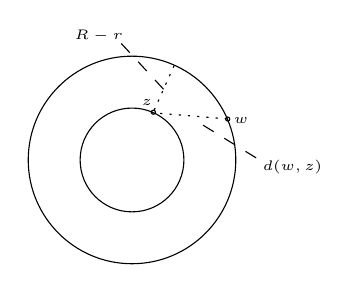
\begin{tikzpicture}[x=0.75pt,y=0.75pt,yscale=-1,xscale=1]
        %uncomment if require: \path (0,300); %set diagram left start at 0, and has height of 300
        
        %Shape: Circle [id:dp4346947048117715] 
        \draw   (200,150) .. controls (200,122.39) and (222.39,100) .. (250,100) .. controls (277.61,100) and (300,122.39) .. (300,150) .. controls (300,177.61) and (277.61,200) .. (250,200) .. controls (222.39,200) and (200,177.61) .. (200,150) -- cycle ;
        %Shape: Circle [id:dp5633091016774019] 
        \draw   (225,150) .. controls (225,136.19) and (236.19,125) .. (250,125) .. controls (263.81,125) and (275,136.19) .. (275,150) .. controls (275,163.81) and (263.81,175) .. (250,175) .. controls (236.19,175) and (225,163.81) .. (225,150) -- cycle ;
        %Straight Lines [id:da044579420049741914] 
        \draw  [dash pattern={on 0.84pt off 2.51pt}]  (270.25,104.56) -- (260.13,127.28) ;
        %Straight Lines [id:da9218408814716863] 
        \draw  [dash pattern={on 0.84pt off 2.51pt}]  (295.8,130.2) -- (260.13,127.28) ;
        %Straight Lines [id:da5249492794602243] 
        \draw  [dash pattern={on 4.5pt off 4.5pt}]  (309.8,149) -- (280.6,131) ;
        %Straight Lines [id:da7471615005961604] 
        \draw  [dash pattern={on 4.5pt off 4.5pt}]  (265.19,115.92) -- (241.8,90.6) ;
        %Shape: Circle [id:dp8921119746382541] 
        \draw   (259.3,127) .. controls (259.3,126.45) and (259.75,126) .. (260.3,126) .. controls (260.85,126) and (261.3,126.45) .. (261.3,127) .. controls (261.3,127.55) and (260.85,128) .. (260.3,128) .. controls (259.75,128) and (259.3,127.55) .. (259.3,127) -- cycle ;
        %Shape: Circle [id:dp188848317748754] 
        \draw   (295.1,130.3) .. controls (295.1,129.75) and (295.55,129.3) .. (296.1,129.3) .. controls (296.65,129.3) and (297.1,129.75) .. (297.1,130.3) .. controls (297.1,130.85) and (296.65,131.3) .. (296.1,131.3) .. controls (295.55,131.3) and (295.1,130.85) .. (295.1,130.3) -- cycle ;
        
        % Text Node
        \draw (257.13,124.88) node [anchor=south] [inner sep=0.75pt]  [font=\tiny]  {$z$};
        % Text Node
        \draw (297.8,133.8) node [anchor=south west] [inner sep=0.75pt]  [font=\tiny]  {$w$};
        % Text Node
        \draw (311.8,157.93) node [anchor=south west] [inner sep=0.75pt]  [font=\tiny]  {$d( w,z)$};
        % Text Node
        \draw (246.8,94.2) node [anchor=south east] [inner sep=0.75pt]  [font=\tiny]  {$R-r$};
        
        
        \end{tikzpicture}
        
        


        \end{center}
        Recall that for a closed set $C$ $d(z,C)=\min_{w\in C}\set{d(w,z)}$. In the case of the disk of radius $R$ we have that 
        $$d(z,\cC)=R-r\geq d(z,w),\word{where}w\in\cC.$$
        This means that 
        $$|w-z|\geq R-r\To\frac{1}{|w-z|}\leq\frac{1}{R-r}.$$
        Now taking the complex modulus of $\rho_N$ for $z$ with $|z|=r$, we have
        $$|\rho_N(z)|\leq\frac{r^n}{2\pi}\oint\limits_\cC\frac{|f(z)|}{|w-z||w|^N}\dd w\leq \frac{r^N}{2\pi}\frac{M}{(R-r)R^N}(2\pi R)=\frac{Mr}{R-r}\left(\frac{r}{R}\right)^{N-1}.$$
        \item It suffices to show that $|\rho_N|\to 0$ as this implies $\rho_N\to0$. Notice that $\frac{r}{R}<1$ because $r<R$. So this means that $\left(\frac{r}{R}\right)^{N-1}<\frac{\eps(R-r)}{rM}$ where $\eps>0$ and $N$ is large enough. Thus for such an $N$ we have 
        $$|\rho_N(z)|\leq \frac{rM}{R-r}\left(\frac{r}{R}\right)^{N-1}<\frac{rM}{R-r}\frac{\eps(R-r)}{rM}=\eps.$$
        We thus conclude that $|\rho_N(z)|\to 0$ as $N\to\infty$ and therefore $\rho_N\to 0$ as well.
    \end{enumerate}
\end{ptcbr}
\begin{Ej}
    For $0\leq r\leq n$, the binomial coefficient $\binom{n}{r}$ is defined by $\binom{n}{r}=\frac{n!}{r!(n-r)!}$.
    \begin{enumerate}[i)]
        \itemsep=-0.4em
        \item Let $\ga=\del B(0,1)$, the positive, circular arc around $0$ with radius $1$. Show that 
        $$\binom{n}{r}=\frac{1}{2\pi i}\oint\limits_\ga \frac{(1+z)^n}{z^{r+1}}\dd z.$$
        \aside{In fact, this works for any simple closed curve around the origin.}
        \item Use the previous item to show that $\binom{n}{r}\leq 2^n$. \emph{This can also be shown directly by computing $(1+1)^n$.}
    \end{enumerate}
\end{Ej}

\begin{ptcbr}
    \begin{enumerate}[i)]
        \itemsep=-0.4em
        \item Notice that the integral in question, by the binomial theorem is: 
        $$\frac{1}{2\pi i}\oint\limits_\ga \frac{1}{z^{r+1}}\left(\sum_{k=0}^{n}\binom{n}{k}z^k\right)\dd z=\frac{1}{2\pi i}\sum_{k=0}^n\binom{n}{k}\oint\limits_{\ga}z^{k-r-1}\dd z.$$
        Notice that most of the terms in the sum are actually zero because %$z^{k-r-1}$ is holomorphic about the origin.
        $$\oint\limits_{\ga}z^{k-r-1}\dd z=(2\pi i)\dl_{kr}.$$
        With this, we have the desired equality as the expression is equal to 
        $$\frac{1}{2\pi i}\binom{n}{r}\oint\limits_{\ga}z^{-1}\dd z=\binom{n}{r}.$$
        \item Now bounding terms in the integral we have that 
        $$\binom{n}{r}\leq\frac{1}{2\pi}(2^n)\text{len}(\ga)=2^n.$$
    \end{enumerate}
\end{ptcbr}
\begin{Ej}[\cite{Stein} 2.7]
    Suppose $f\:\bD\to\bC$ is holomorphic. Show that the diameter $d=\sup_{z,w\in\bD}|f(z)-f(w)|$ of the image of $f$ satisfies $2|f'(0)|\leq d$.\par
    Moreover, it can be shown that equality holds precisely when $f$ is linear, $f(z)=az+b$.
    \aside{In connection with this result, see the relationship between the diameter of a curve and Fourier series described in Problem 1, Chapter 4, Book I.}
    \hint{$2f'(0)=\frac{1}{2\pi i}\oint\limits_{|\ze|=r}\frac{f(\ze)-f(-\ze)}{\ze^2}\dd\ze$ when $0<r<1$.}
\end{Ej}
%https://math.stackexchange.com/questions/1375438/stein-shakarchi-complex-analysis-ch-2-ex-7?noredirect=1&lq=1
\begin{ptcbr}
    To show the desired identity for $f'(0)$ it suffices to use Cauchy's formula:
    $$f'(z)=\frac{1}{2\pi i}\oint\limits_{|w|=r}\frac{f(w)}{(w-z)^2}\dd w\To f'(0)=\frac{1}{2\pi i}\oint\limits_{|w|=r}\frac{f(w)}{w^2}\dd w.$$
    Now take the change of variable $w=-u\To \dd w=-\dd u$. The curve through which we are integrating remains the same, as $|w|=|-u|=|u|$. Thus 
    $$f'(0)=\frac{1}{2\pi i}\oint\limits_{|u|=r}\frac{-f(u)}{u^2}\dd u.$$
    Renaming variables and adding the last two results we get 
    $$2f'(0)=\frac{1}{2\pi i}\oint\limits_{|\ze|=r}\frac{f(\ze)-f(-\ze)}{\ze^2}\dd\ze.$$
    Taking the complex modulus we see that 
    $$2|f'(0)|\leq\frac{1}{2\pi}\oint\limits_{|\ze|=r}\frac{|f(\ze)-f(-\ze)|}{|\ze|^2}\dd\ze\leq \frac{1}{2\pi r^2}\sup_{|\ze|=r}|f(\ze)-f(-\ze)|(2\pi r)$$
    As $\set{|\ze|=r}\subseteq\bD$ we have that 
    $$\sup_{|\ze|=r}|f(\ze)-f(-\ze)|\leq d\To 2|f'(0)|\leq\frac{d}{r}.$$
    As the last inequality holds for all $0<r<1$, in particular we have that 
    $$|f'(0)|\leq\inf_{0<r<1}\frac{d}{r}=d$$
    which is the desired inequality.
    %https://math.stackexchange.com/questions/3619008/2-leftf0-right-sup-z-omega-in-mathbbd-leftfz-f-omega-right?noredirect=1&lq=1
    %https://math.stackexchange.com/questions/339569/a-result-similar-to-schwarz-lemma
    %http://manetheren.bigw.org/~ray/diampblm.pdf
\end{ptcbr}
\begin{Ej}
    Let $\Om$ be a bounded open subset of $\bC$, and $\vf\:\Om\to\Om$ a holomorphic function. Prove that if there exists a point $z_0\in\Om$ such that $\vf(z_0)=z_0$ and $\vf'(z_0)=1$,
    then $\vf$ is linear.
\hint{Why can one assume that $z_0=0$? Write $z+a_nz^n+O(z^{n+1})$ near $0$, and prove that if $\vf_k=\vf\circ\vf\circ\dots\circ\vf$ (where $\vf$ appears $k$ times), then $\vf_k(z)=ka_nz^n+O(z^{n+1})$. Apply the Cauchy inequalities and let $k\to\infty$ to conclude the proof.}
\end{Ej}

\begin{ptcbr}
    %https://math.stackexchange.com/questions/275270/holomorphic-function-varphi-with-fixed-point-z-0-such-that-varphiz-o-1
   Let us begin by making some observations:
   \begin{itemize}
    \itemsep=-0.4em
    \item As $\vf$ is holomorphic inside $\Om$, it is analytic inside $\Om$ and thus we may write it as a power series centered at $z_0$
    $$\vf(z)=\sum_{n\geq 0}^{}a_n(z-z_0)^n.$$
    The conditions in the problem imply that $a_0=z_0$ and $a_1=1$ which means that 
    $$\vf(z)=z_0+(z-z_0)+\sum_{n\geq 2}^{}a_n(z-z_0)^n.$$
   \end{itemize}
\end{ptcbr}

\section{Day 11| 20230213}

We have used the Cauchy integral formula for derivatives. As a corollary we have that 

\begin{Cor}
    If $f$ is holomorphic about $z_0\in\Om$, then $f$ is analytic at $z_0$.
\end{Cor}

\begin{Th}
    Suppose $f$ is holomorphic on a domain $\Om$ with $(z_n)\subseteq\Om$ such that $z_n\to z_0\in\Om$. Suppose that $f(z_n)=0$ for all $n$, then $f$ is identically zero.
\end{Th}

\begin{ptcbp}
    About $z_0$ we have 
    $$f(z)=\sum_{n\geq m}^{}a_n(z-z_0)^n=(z-z_0)^m\sum_{n\geq m}^{}a_n(z-z_0)^{n-m}=(z-z_0)^mg(z),\ a_m\neq 0.$$
    We also have that $g(z_0)=a_m\neq 0$. As $g$ is holomorphic, $|z-z_0|<\eps$ implies $g(z)\neq 0$. But for large enough $k$, if $|z_k-z_0|<\eps$, if $f(z_k)=0$, then 
    $$f(z_k)=(z_k-z_0)^mg(z_k).$$
\end{ptcbp}

\begin{Th}
    Suppose $f,g$ are holomorphic on a domain $\Om$. Suppose also that there is a non-constant sequence $(z_n)\subseteq\Om$ such that $z_n\to z\in\Om$ and $f(z_n)=g(z_n)$. Then $f=g$.
\end{Th}

\begin{ptcbp}
    Letting $h=f-g$, we see that $h$ is identically zero with the previous result so $f=g$.
\end{ptcbp}

\begin{Def}
    We say a that a sequence of functions $(f_n)$ converges to $f$ pointwise on $S$, if 
    $$\forall z(f_n(z)\xrightarrow[]{n\to\infty} f(z)).$$
    Meanwhile the convergence is uniform if 
    $$\norm{f_n-f}_\infty\xrightarrow[]{n\to\infty}0.$$
\end{Def}

\begin{Ex}
    The sequence of functions $(z^n)$ converges pointwise to $\dl_{z0}$ which is not continuous. Uniform convergence preserves continuity so $(z^n)$ is not uniformly convergent.\par
    Power series converge uniformly.
\end{Ex}
%%%%%%%%%%%% Contents end %%%%%%%%%%%%%%%%
\ifx\nextra\undefined
\printindex
\else\fi
\nocite{*}
\bibliographystyle{plain}
\bibliography{bibiComAnal.bib}
\end{document} 
